\documentclass[letterpaper,12pt]{article}   %%% Can be report

%% set paper margins
\oddsidemargin=0.1in
\evensidemargin=0.1in
\textwidth=6.0in
\topmargin=-0.7in
\textheight=9.0in
\parindent=0.2in

\usepackage{amsmath,amssymb,bm}
\usepackage{graphicx}
\usepackage{rotating}
\usepackage{subfigure}
\graphicspath{%
  {figs/ipe/}
  {figs/dia/}
  {figs/matlab/}
  {figs/imag/}
} 
\usepackage[width=11cm,font=footnotesize,labelfont=bf, %
format=default,justification=centerlast]{caption} % Figure caption text customization 

\usepackage{pgfgantt}

\usepackage{booktabs,array} % Packages for tables

\usepackage{hyperref}
\usepackage{soul}
\usepackage{setspace}
\usepackage{multirow}

\usepackage[ruled, vlined, linesnumbered]{algorithm2e} % For algorithms

\usepackage{tikz}
\usetikzlibrary{positioning,fit}

\usepackage{siunitx}
\sisetup{unitsep=\cdot}

\title{ECE498:~Senior Capstone Project I\\\textbf{\underline{Project Proposal}}\\
\vspace{0.5in}
Project Title: Robotic Cart
\vspace{1.0in}
\author{Kallistah Allen, Darrah Beebe and Jason Braker\\ Advisors: Dr.~Suruz Miah and Dr.~Prasad Shastry}
}
%\date{February 6, 2003}  No need to write, Date will be automatically on the title page
\date{}  % Do not show date on the title page

%%%%%%%%%%%%%%%%% Set document line spacing %%%%%%%%%%%%%%%%%%%%%
\singlespacing
%\onehalfspacing
%\doublespacing
% all packages are in the following tex file.
%\input{paper-preamble.tex}
\begin{document}

%%% Make title page 
\begin{titlepage}
 \maketitle

\vspace*{4.0cm}
\begin{center}
\normalsize
Electrical and Computer Engineering Department\\
Caterpillar College of Engineering and Technology\\
\href{http://www.bradley.edu/}{Bradley University}\\

\vspace*{6.0cm}
\copyright~K.~Allen,~D.~Beebe~and~J.~Braker, Peoria, IL, USA, 2020\\

\end{center}
\thispagestyle{empty}

\end{titlepage} 
%%%%%%%%%%%%
%\thispagestyle{empty}
%\maketitle
\newpage
\renewcommand{\contentsname}{Table of Contents}
\tableofcontents
\newpage

\section{Introduction}
Robotic carts are a prevalent invention designed to aid the customer in a number of important indoor and outdoor tasks. There are systems currently on the market that perform these tasks in a variety of ways. For example, in a grocery store, a customer may require the need of more than one cart but cannot push or pull two carts simultaneously. One major drawback however is that people with disabilities cannot push one cart let alone have a second cart to carry more items. In this project, we are proposing a robotic cart that would primarily use analog signals with the use of cost-effective wireless communication to identify the customer and be able to track and follow the customer through the store. This implementation of a fully functional robotic cart will outreach the scope of the project but is the overall goal for this project in the coming years while encouraging further research into this field. Applications of this system include mail delivery carts, file transferring carts in offices, hospital carts to aid nurses and doctors by carrying medicine or surgery supplies, and use in construction sites to carry tools and other supplies across the job site.

\section{Literature Review}
Abundant research in the field of robotic carts shows various ways in which to implement a system that will help consumers with carrying groceries through stores (see~\cite{Rawashdeh2017-Person},~\cite{islam_lam_fukuda_kobayashi_kuno_2019},~\cite{Sales2016-CompaRob}). Currently, the work being done focuses on a few different methods of having the robotic cart interface with the customer and follow them through the store. A mobile platform interface that implements ultrasound and radio transmissions technology is one such method that has been utilized to follow a customer through a store~\cite{Sales2016-CompaRob}. Another method that has been implemented is the use of a GRU (Gated Recurrent Unit) network to detect shopping habits of customers while also using a LiDAR sensor and camera to detect and map the customer using a two-dimensional skeleton and follow them through the store~\cite{islam_lam_fukuda_kobayashi_kuno_2019}. In the last method, the authors utilized an Arduino MEGA 2560, six ultrasonic sensors, two DC motors with PWM (Pulse Width Modulation), an Android Studio IDE device, and Bluetooth in order to detect the customer and follow them through the store~\cite{Rawashdeh2017-Person}. In our project we are implementing XBee S2C RF radios, which are inexpensive and easily configurable, as a remote that the robot will be able to track instead of using line of sight methods~\cite{Miah2018-Intelligent}. In addition to the XBee S2C RF radios we will equip the robot with a parabolic reflector, which improves Wi-Fi reception at various distances and angles, based on research done previously in this type of robot localization and mapping~\cite{Miah2018-Intelligent}~\cite{Li2013ANA}. This approach also requires understanding of multipath interference which is common in Wi-Fi based wireless positioning sensing systems. Some methods, seen in~\cite{xie_jiang_zhao_zhang_2019}, explains that using course estimation calculations such as received signal strength indicator (RSSI) and time difference of arrival (TDoA) is key to compensate for the multipath interference in received signals.~\cite{ladd_bekris_rudys_kavraki_wallach_2005} shows a different approach to the multipath issue by using an IEEE 802.11b wireless Ethernet device to measure RF signals. This device system was used because it is communicable between a mobile device and a localization based service with low complexity for the user. Also, in~\cite{lindhe_johansson_bicchi_2007} the research states several other ways to counteract the multipath fading with methods such as antenna diversity, frequency spreading, or adaptive antenna arrays. The method used in this paper was to sample the radio signal strength (RSS) at discrete points without too much deviation from the robot's desired position in an indoor environment. Lastly, in~\cite{Lindhe2009} the method that is utilized exploits multipath fading by measuring the signal-to-noise ratio (SNR) and adjusting the robot's motion to spend more time where the channel strength is greater.

\vspace*{12pt}
\noindent
In this project we aim to use the XBee S2C RF radios and a parabolic reflector combined into a rotating system similar to the one presented in~\cite{Miah2018-Intelligent} in order to have the robot track the customer through a store. The major challenge of this implementation will be estimating the distance between the robot and the remote in varying environments without using line of sight sensing.

\section{System Requirements}
There are three requirements for our system. The first requirement is that the cart should be able to follow the remote while maintaining a distance of 1 to 1.5 meters. This requirement comes from the intended usage of the project, which is a cart that follows the user. The cart must be able to follow the remote, but it also must be able to keep an appropriate distance so it does not run into the user or fall too far behind.

\vspace*{12pt}
\noindent
The second requirement for the system is that the cart should be able to travel at 1 m/s. If the cart can only travel slowly, it will not be as useful since the user will have to walk very slowly to allow the cart to keep up.

\vspace*{12pt}
\noindent
The third requirement is that line-of-sight communication between the cart and the robot must not be required. In the case that an obstacle gets between the cart and the remote, the communication should be able to be maintained so that the cart still knows where the user is located.

\section{System Architecture}
The system for this project consists of two subsystems which are the Mobile Cart and the Remote Target. as seen in Figure \ref{fig:sys_block_diag}. The Mobile Cart system is a wheeled robot that sends and receives radio signals to follow the remote target. The Remote Target acts as the target for the Mobile Cart in the system by sending radio signals back and forth with the cart.

\subsection{System Block Diagram}
The block diagram of the overall system is shown in \autoref{fig:sys_block_diag}. There are four inputs to the system. The system must have a power source, which will be a battery. There will be an on/off switch to allow the system to be powered down when not in use. The motion of the cart will be controlled by the motion of the remote. A stretch goal is to have mode selection buttons to allow the user to put the system into different operating modes.

\vspace*{12pt}
\noindent
The main output of the system is the trajectory of the cart. As the user moves with the remote, the cart will move to follow the user. The other output of the system is status indication in the form of LED lights. These lights will be used to notify the user of the status of the system.

\begin{figure}[!h]
    \centering
    
\includegraphics[scale=0.9]{figs/system_block_diagram_2}
    \caption{System level block diagram detailing inputs and outputs to the system}
	\label{fig:sys_block_diag}
\end{figure}

\subsection{Subsystem Block Diagrams}
Both of the subsystems of the mobile cart system, being the Mobile Cart and Remote Target, act as their own enclosed systems. The two subsystems communicate with one another by relaying radio messages between them. The block diagram of the Remote Target subsystem is shown in \autoref{fig:remote_block_diag}. Of the two subsystems the Remote Target is the simplest since it only requires an XBee module attached to a 9 volt battery with a voltage regulation circuit.

\vspace*{12pt}
\noindent
The Mobile Cart subsystem block diagram is shown in \autoref{fig:mobile_block_diag}. The Mobile Cart has four inputs. The cart requires a power source, which will be a Li-Po battery. The power to the subsystem will be toggled by an on/off switch. The buttons for changing the operating mode of the cart will be on the cart if we have time to implement them. The final input to the mobile cart subsystem is the XBee network messages received from the remote target.

\vspace*{12pt}
\noindent
There are three outputs of the mobile cart subsystem. The first is the wheel velocities that move the cart. There will also be LEDs to indicate the status of the system to the user. Also, the cart will send radio messages to the remote target by means of an array of XBee radio modules.

\begin{figure}[h!]
  \centering
  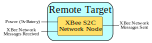
\includegraphics[scale=0.9]{figs/remote_target_block_diagram}
  \caption{Remote Target block diagram}
  \label{fig:remote_block_diag}
\end{figure}

\begin{figure}[h!]
  \centering
  \includegraphics[scale=0.82]{figs/mobile_cart_block_diagram}
  \caption{Mobile Robot block diagram}
  \label{fig:mobile_block_diag}
\end{figure}

\subsection{System Components}
There are several components that are required for the mobile cart system. Although some of these parts are available in the Bradley University laboratory, other parts must be purchased. The parts that exist in the lab are shown in \autoref{tab:Partslablist}. Also, \autoref{tab:Partslist} shows the list of parts that we must purchase. The parts lists shown are the parts needed to build two copies of the mobile cart system.

\begin{table}[h!]
  \centering
  \begin{tabular}{c|c}
      \toprule
      \textbf{Quantity} & \textbf{Parts}\\
      \toprule
      2 & Budget Bot Chassis\\
      4 & 10 uF Ceramic Capacitor\\
      4 & LM1117 Regulator\\
      2 & Battery Packs for Budget Bot\\
      8 & 9V Batteries\\
      4 & Solderable PCB Boards\\
      3 & XBee USB Adapter\\
      \bottomrule
      %\multicolumn{2}{r|}{\textbf{Total}} & \$ 562.34\\
      %\bottomrule
  \end{tabular}
  \caption{Parts Available in Laboratory}
  \label{tab:Partslablist}
\end{table}

\begin{table}[h!]
  \centering
  \begin{tabular}{c|c|c}
    \toprule
    \textbf{Quantity} & \textbf{Parts} & \textbf{Price}\\
    \toprule
    4 & Pololu 37D Metal Gaermotor 4751 & \$ 39.95\\
    12 & XBee S2C Module & \$ 23.10\\
    10 & XBee Adapter Board & \$ 4.99\\
    2 & Twotrees 4 Lead Nema 17 Stepper Motor & \$ 9.99\\
    1 & 4-Pin JST SH Connector - 20 Pack & \$ 7.99\\
    1 & 6-Pin JST SH Connector - 10 Pack & \$ 9.99\\
    1 & Aluminum Foil Tape - 2 in x 5 yd & \$ 6.05\\
    \bottomrule
    \multicolumn{2}{r|}{\textbf{Total}} & \$ 562.34\\
    \bottomrule
  \end{tabular}
  \caption{Purchased parts for the Robotic Cart Project}
  \label{tab:Partslist}
\end{table}

\vspace*{12pt}
\noindent
The main components of the system are the Budget Bot Chassis (\autoref{fig:budgetBotChassis}), the BeagleBone Blue embedded computer (\autoref{fig:beagleboneBlue}), and the XBee S2C Modules (\autoref{fig:XBeeModule}). Another major component is the reflector array that will be used to directionalize the signals coming from the remote.

\begin{figure}
  \centering
  \begin{minipage}[t]{0.32\textwidth}
    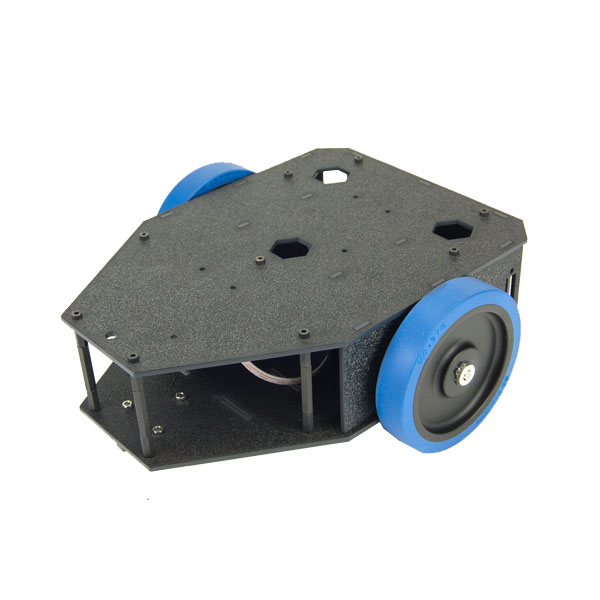
\includegraphics[width=1\textwidth]{figs/img/budgetbot_chassis}
    \captionsetup{width=\textwidth}
    \caption{Budget Bot Chassis}
    \label{fig:budgetBotChassis}
  \end{minipage}%
  \begin{minipage}[t]{0.32\textwidth}
    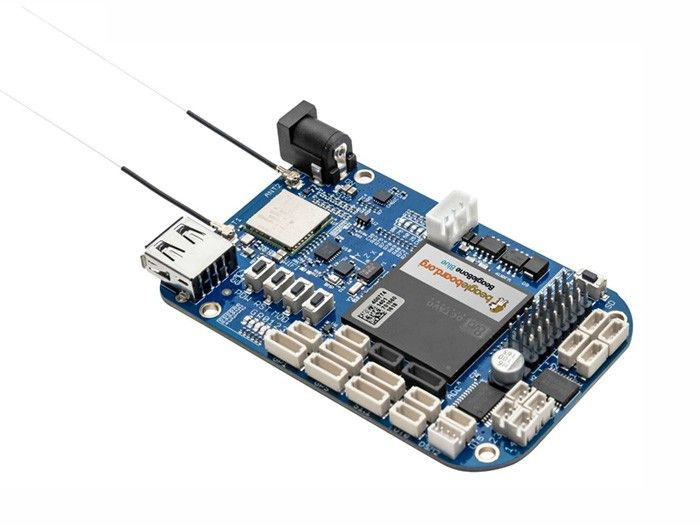
\includegraphics[width=1\textwidth]{figs/img/beaglebone_blue}
    \captionsetup{width=\textwidth}
    \caption{BeagleBone Blue}
    \label{fig:beagleboneBlue}
  \end{minipage}
  \begin{minipage}[t]{0.32\textwidth}
    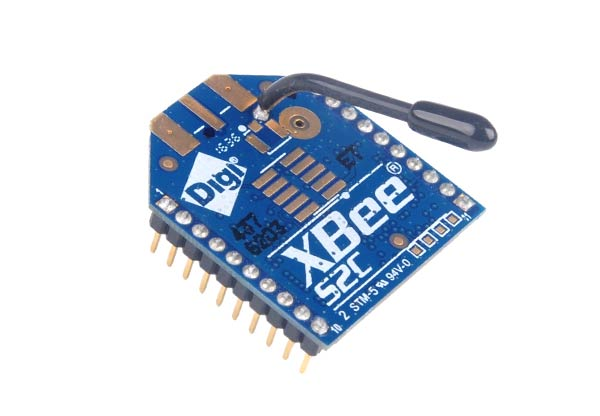
\includegraphics[width=1\textwidth]{figs/img/Xbee-S2C-Module}
    \captionsetup{width=\textwidth}
    \caption{XBee S2C Module}
    \label{fig:XBeeModule}
  \end{minipage}
\end{figure}

\vspace*{12pt}
\noindent
Two reflector designs will be evaluated in this project. The first, shown in \autoref{fig:parabolodialReflector}, is a paraboloidal reflector. This design maximizes the signal strength of signals that come head-on into the reflector. Since the remote will be carried by the user, it is likely that it will be positioned at a higher altitude than the reflector array. The paraboloidal reflector design may not be able to pick up the signals from the remote as well because of this. To solve this problem, we designed a combination parabolic/paraboloidal reflector, as shown in \autoref{fig:parabolicReflector}. The lower part of this reflector is paraboloidal in shape to limit the signals coming from below. The upper part of the reflector is strictly parabolic. This shape focuses the signals in the horizontal plane, but allows signals from above to still be picked up. We plan to construct both of these reflector types by 3d printing the frames, then lining them with reflective foil tape. Both models will then be tested to determine which design works better.

\begin{figure}[h!]
  \centering
  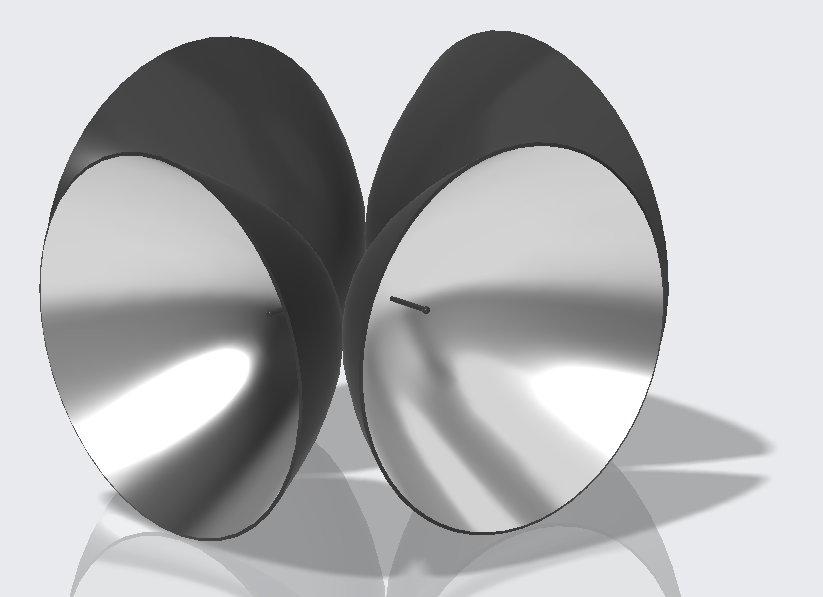
\includegraphics[width=4in]{figs/img/paraboloidalReflector}
  \caption{Paraboloidal Reflector Model}
  \label{fig:parabolodialReflector}
\end{figure}

\begin{figure}[h!]
  \centering
  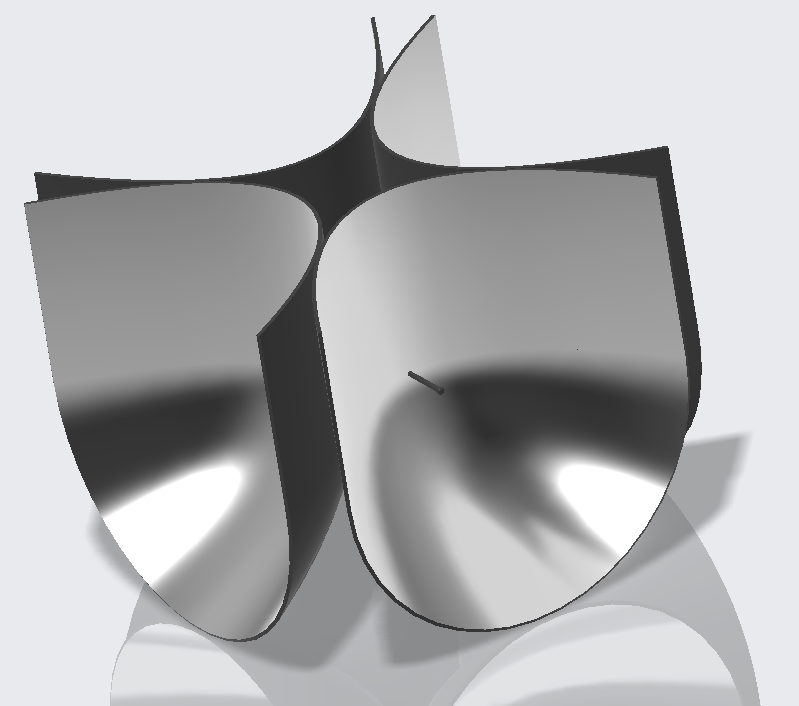
\includegraphics[width=4in]{figs/img/parabolicReflector}
  \caption{Combined Parabolic/Paraboloidal Reflector}
  \label{fig:parabolicReflector}
\end{figure}

\subsection{System Operation}
The control of the Mobile Cart will be handled by a central embedded computer, which will be a BeagleBone Blue. Two DC motors will be used to drive wheels to move the cart. Five XBee modules will be used to allow communication with the remote target. One of these radio sensors will be mounted on top of the cart to broadcast in all directions. The other four sensors will be placed inside parabolic reflectors at right angles to each other. This sensor array will be mounted on a stepper motor to allow rotation. 

\vspace*{12pt}
\noindent
The strength of the radio signals between the cart and remote will be used to estimate the position of the remote relative to the cart. By rotating the sensor array 90 degrees and measuring the signal strength of messages from the remote at several steps in the rotation, the bearing of the remote can be estimated as the direction in which the maximum signal strength is received. To estimate the distance between the cart and the remote, the signal strength will be measured and used to calculate the distance. The omnidirectional radio module on top will be responsible for coordinating the messages from the remote by sending the remote commands that tell the remote when to send signals.

\subsection{Navigation Algorithm}
Once the bearing and distance of the remote are estimated, the cart must move to follow the remote. We will use a modified Point Navigation algorithm to navigate the robot to follow the remote. The robot will estimate the coordinates of the remote with respect to the robot's local reference frame. The robot will then apply actuation to move to the point that is a set following distance from the remote. A high-level flowchart of the algorithm is shown in \autoref{fig:navAlgoFlowchart}. Also, a more detailed pseudo-code version of the algorithm is shown in \autoref{alg:navAlgo}.

\begin{figure}
  \centering
  % Graphic for TeX using PGF
% Title: S:\Senior Project\seniorProject2-2020-21-Docs\figs\dia\algorithmFlowchart.dia
% Creator: Dia v0.97.2
% CreationDate: Thu Nov 19 10:16:16 2020
% For: Jason Braker
% \usepackage{tikz}
% The following commands are not supported in PSTricks at present
% We define them conditionally, so when they are implemented,
% this pgf file will use them.
\ifx\du\undefined
  \newlength{\du}
\fi
\setlength{\du}{15\unitlength}
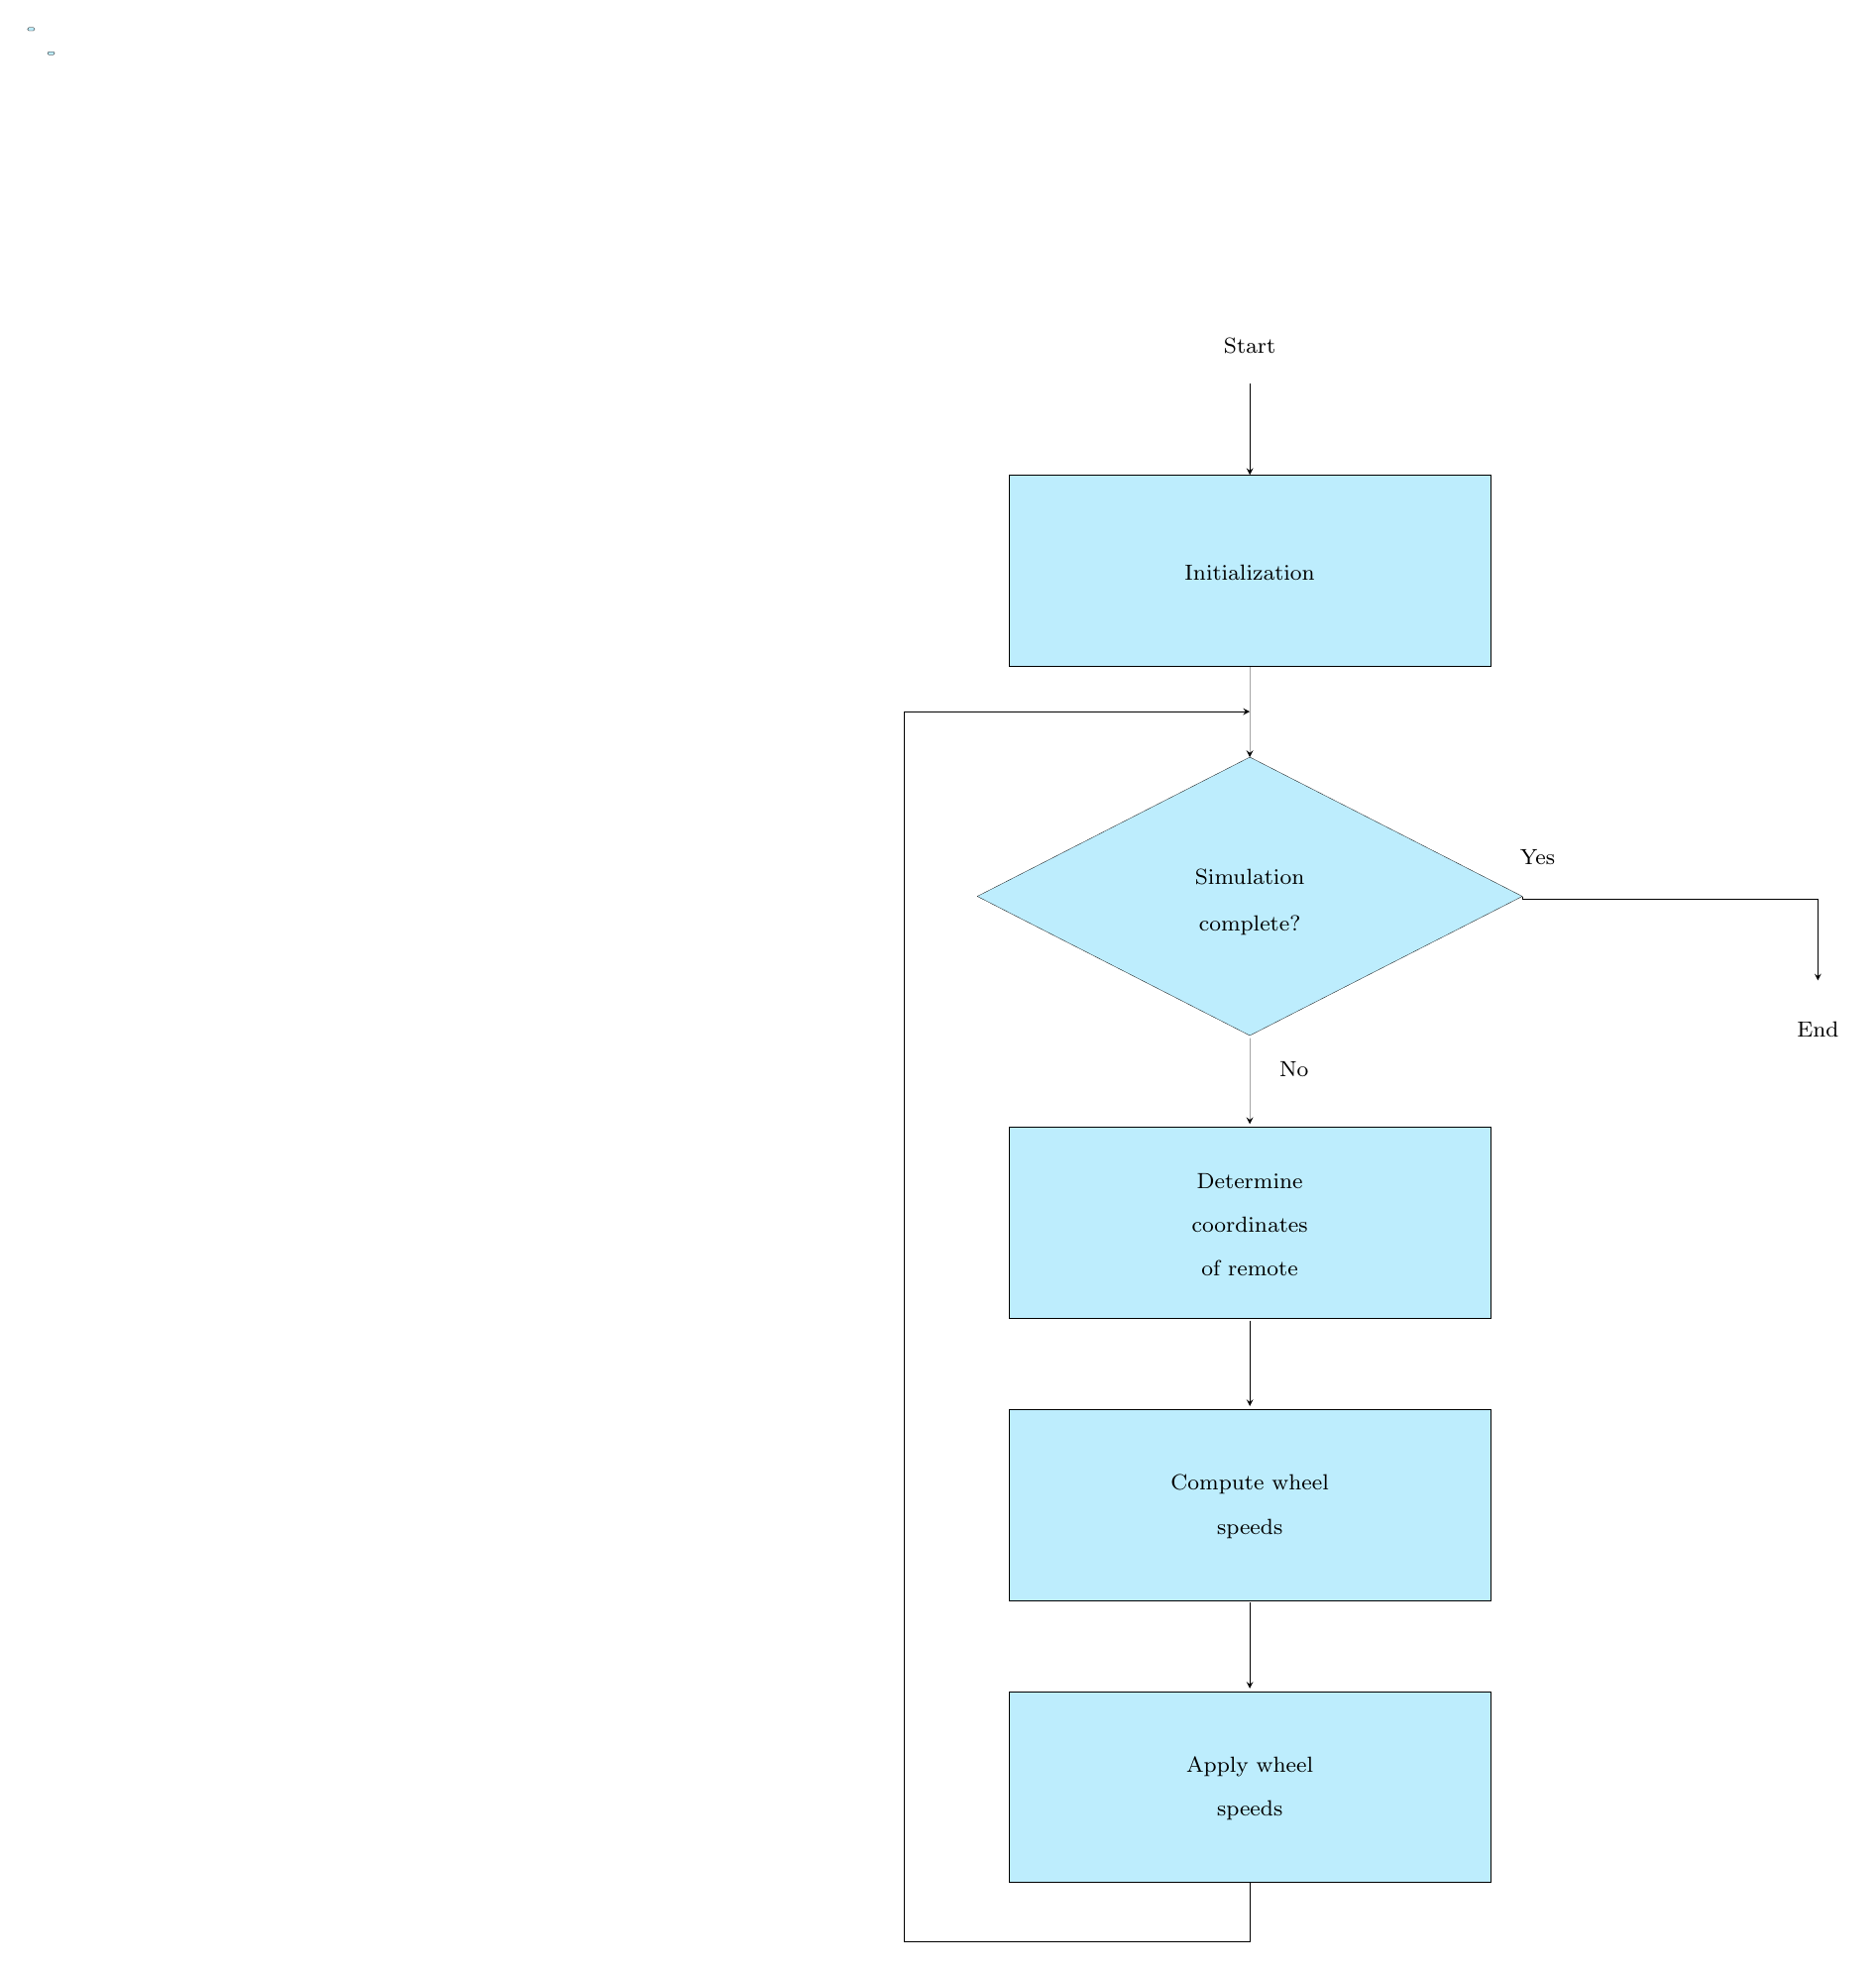
\begin{tikzpicture}[scale=0.7, font=\footnotesize]
\pgftransformxscale{1.000000}
\pgftransformyscale{-1.000000}
\definecolor{dialinecolor}{rgb}{0.000000, 0.000000, 0.000000}
\pgfsetstrokecolor{dialinecolor}
\definecolor{dialinecolor}{rgb}{1.000000, 1.000000, 1.000000}
\pgfsetfillcolor{dialinecolor}
\pgfsetlinewidth{0.100000\du}
\pgfsetdash{}{0pt}
\pgfsetdash{}{0pt}
\pgfsetbuttcap
\pgfsetmiterjoin
\pgfsetlinewidth{0.100000\du}
\pgfsetbuttcap
\pgfsetmiterjoin
\pgfsetdash{}{0pt}
\definecolor{dialinecolor}{rgb}{0.741176, 0.929412, 0.992157}
\pgfsetfillcolor{dialinecolor}
\pgfpathmoveto{\pgfpoint{21.890567\du}{5.100000\du}}
\pgfpathlineto{\pgfpoint{24.357233\du}{5.100000\du}}
\pgfpathcurveto{\pgfpoint{24.697809\du}{5.100000\du}}{\pgfpoint{24.973900\du}{5.458172\du}}{\pgfpoint{24.973900\du}{5.900000\du}}
\pgfpathcurveto{\pgfpoint{24.973900\du}{6.341828\du}}{\pgfpoint{24.697809\du}{6.700000\du}}{\pgfpoint{24.357233\du}{6.700000\du}}
\pgfpathlineto{\pgfpoint{21.890567\du}{6.700000\du}}
\pgfpathcurveto{\pgfpoint{21.549991\du}{6.700000\du}}{\pgfpoint{21.273900\du}{6.341828\du}}{\pgfpoint{21.273900\du}{5.900000\du}}
\pgfpathcurveto{\pgfpoint{21.273900\du}{5.458172\du}}{\pgfpoint{21.549991\du}{5.100000\du}}{\pgfpoint{21.890567\du}{5.100000\du}}
\pgfusepath{fill}
\definecolor{dialinecolor}{rgb}{0.000000, 0.000000, 0.000000}
\pgfsetstrokecolor{dialinecolor}
\pgfpathmoveto{\pgfpoint{21.890567\du}{5.100000\du}}
\pgfpathlineto{\pgfpoint{24.357233\du}{5.100000\du}}
\pgfpathcurveto{\pgfpoint{24.697809\du}{5.100000\du}}{\pgfpoint{24.973900\du}{5.458172\du}}{\pgfpoint{24.973900\du}{5.900000\du}}
\pgfpathcurveto{\pgfpoint{24.973900\du}{6.341828\du}}{\pgfpoint{24.697809\du}{6.700000\du}}{\pgfpoint{24.357233\du}{6.700000\du}}
\pgfpathlineto{\pgfpoint{21.890567\du}{6.700000\du}}
\pgfpathcurveto{\pgfpoint{21.549991\du}{6.700000\du}}{\pgfpoint{21.273900\du}{6.341828\du}}{\pgfpoint{21.273900\du}{5.900000\du}}
\pgfpathcurveto{\pgfpoint{21.273900\du}{5.458172\du}}{\pgfpoint{21.549991\du}{5.100000\du}}{\pgfpoint{21.890567\du}{5.100000\du}}
\pgfusepath{stroke}
% setfont left to latex
\definecolor{dialinecolor}{rgb}{0.000000, 0.000000, 0.000000}
\pgfsetstrokecolor{dialinecolor}
\node at (23.123900\du,6.00000\du){Start};
\definecolor{dialinecolor}{rgb}{0.741176, 0.929412, 0.992157}
\pgfsetfillcolor{dialinecolor}
\fill (23.123842\du,13.536900\du)--(28.113283\du,16.085084\du)--(23.123842\du,18.633268\du)--(18.134400\du,16.085084\du)--cycle;
\pgfsetlinewidth{0.100000\du}
\pgfsetdash{}{0pt}
\pgfsetdash{}{0pt}
\pgfsetmiterjoin
\definecolor{dialinecolor}{rgb}{0.000000, 0.000000, 0.000000}
\pgfsetstrokecolor{dialinecolor}
\draw (23.123842\du,13.536900\du)--(28.113283\du,16.085084\du)--(23.123842\du,18.633268\du)--(18.134400\du,16.085084\du)--cycle;
% setfont left to latex
\definecolor{dialinecolor}{rgb}{0.000000, 0.000000, 0.000000}
\pgfsetstrokecolor{dialinecolor}
\node at (23.123842\du,15.725084\du){Simulation};
% setfont left to latex
\definecolor{dialinecolor}{rgb}{0.000000, 0.000000, 0.000000}
\pgfsetstrokecolor{dialinecolor}
\node at (23.123842\du,16.625084\du){complete?};
\definecolor{dialinecolor}{rgb}{0.741176, 0.929412, 0.992157}
\pgfsetfillcolor{dialinecolor}
\fill (18.709600\du,20.301700\du)--(18.709600\du,23.801700\du)--(27.538230\du,23.801700\du)--(27.538230\du,20.301700\du)--cycle;
\pgfsetlinewidth{0.100000\du}
\pgfsetdash{}{0pt}
\pgfsetdash{}{0pt}
\pgfsetmiterjoin
\definecolor{dialinecolor}{rgb}{0.000000, 0.000000, 0.000000}
\pgfsetstrokecolor{dialinecolor}
\draw (18.709600\du,20.301700\du)--(18.709600\du,23.801700\du)--(27.538230\du,23.801700\du)--(27.538230\du,20.301700\du)--cycle;
% setfont left to latex
\definecolor{dialinecolor}{rgb}{0.000000, 0.000000, 0.000000}
\pgfsetstrokecolor{dialinecolor}
\node at (23.123915\du,21.291700\du){Determine};
% setfont left to latex
\definecolor{dialinecolor}{rgb}{0.000000, 0.000000, 0.000000}
\pgfsetstrokecolor{dialinecolor}
\node at (23.123915\du,22.091700\du){coordinates};
% setfont left to latex
\definecolor{dialinecolor}{rgb}{0.000000, 0.000000, 0.000000}
\pgfsetstrokecolor{dialinecolor}
\node at (23.123915\du,22.891700\du){of remote};
\pgfsetlinewidth{0.100000\du}
\pgfsetdash{}{0pt}
\pgfsetdash{}{0pt}
\pgfsetbuttcap
\pgfsetmiterjoin
\pgfsetlinewidth{0.100000\du}
\pgfsetbuttcap
\pgfsetmiterjoin
\pgfsetdash{}{0pt}
\definecolor{dialinecolor}{rgb}{0.741176, 0.929412, 0.992157}
\pgfsetfillcolor{dialinecolor}
\pgfpathmoveto{\pgfpoint{32.290567\du}{17.675000\du}}
\pgfpathlineto{\pgfpoint{34.757233\du}{17.675000\du}}
\pgfpathcurveto{\pgfpoint{35.097809\du}{17.675000\du}}{\pgfpoint{35.373900\du}{18.033172\du}}{\pgfpoint{35.373900\du}{18.475000\du}}
\pgfpathcurveto{\pgfpoint{35.373900\du}{18.916828\du}}{\pgfpoint{35.097809\du}{19.275000\du}}{\pgfpoint{34.757233\du}{19.275000\du}}
\pgfpathlineto{\pgfpoint{32.290567\du}{19.275000\du}}
\pgfpathcurveto{\pgfpoint{31.949991\du}{19.275000\du}}{\pgfpoint{31.673900\du}{18.916828\du}}{\pgfpoint{31.673900\du}{18.475000\du}}
\pgfpathcurveto{\pgfpoint{31.673900\du}{18.033172\du}}{\pgfpoint{31.949991\du}{17.675000\du}}{\pgfpoint{32.290567\du}{17.675000\du}}
\pgfusepath{fill}
\definecolor{dialinecolor}{rgb}{0.000000, 0.000000, 0.000000}
\pgfsetstrokecolor{dialinecolor}
\pgfpathmoveto{\pgfpoint{32.290567\du}{17.675000\du}}
\pgfpathlineto{\pgfpoint{34.757233\du}{17.675000\du}}
\pgfpathcurveto{\pgfpoint{35.097809\du}{17.675000\du}}{\pgfpoint{35.373900\du}{18.033172\du}}{\pgfpoint{35.373900\du}{18.475000\du}}
\pgfpathcurveto{\pgfpoint{35.373900\du}{18.916828\du}}{\pgfpoint{35.097809\du}{19.275000\du}}{\pgfpoint{34.757233\du}{19.275000\du}}
\pgfpathlineto{\pgfpoint{32.290567\du}{19.275000\du}}
\pgfpathcurveto{\pgfpoint{31.949991\du}{19.275000\du}}{\pgfpoint{31.673900\du}{18.916828\du}}{\pgfpoint{31.673900\du}{18.475000\du}}
\pgfpathcurveto{\pgfpoint{31.673900\du}{18.033172\du}}{\pgfpoint{31.949991\du}{17.675000\du}}{\pgfpoint{32.290567\du}{17.675000\du}}
\pgfusepath{stroke}
% setfont left to latex
\definecolor{dialinecolor}{rgb}{0.000000, 0.000000, 0.000000}
\pgfsetstrokecolor{dialinecolor}
\node at (33.523900\du,18.515000\du){End};
\pgfsetlinewidth{0.100000\du}
\pgfsetdash{}{0pt}
\pgfsetdash{}{0pt}
\pgfsetbuttcap
{
\definecolor{dialinecolor}{rgb}{0.000000, 0.000000, 0.000000}
\pgfsetfillcolor{dialinecolor}
% was here!!!
\pgfsetarrowsend{stealth}
\definecolor{dialinecolor}{rgb}{0.000000, 0.000000, 0.000000}
\pgfsetstrokecolor{dialinecolor}
\draw (23.123900\du,6.700000\du)--(23.123900\du,8.368440\du);
}
\pgfsetlinewidth{0.100000\du}
\pgfsetdash{}{0pt}
\pgfsetdash{}{0pt}
\pgfsetbuttcap
{
\definecolor{dialinecolor}{rgb}{0.000000, 0.000000, 0.000000}
\pgfsetfillcolor{dialinecolor}
% was here!!!
\pgfsetarrowsend{stealth}
\definecolor{dialinecolor}{rgb}{0.000000, 0.000000, 0.000000}
\pgfsetstrokecolor{dialinecolor}
\draw (23.123900\du,11.868400\du)--(23.123800\du,13.536900\du);
}
\pgfsetlinewidth{0.100000\du}
\pgfsetdash{}{0pt}
\pgfsetdash{}{0pt}
\pgfsetbuttcap
{
\definecolor{dialinecolor}{rgb}{0.000000, 0.000000, 0.000000}
\pgfsetfillcolor{dialinecolor}
% was here!!!
\pgfsetarrowsend{stealth}
\definecolor{dialinecolor}{rgb}{0.000000, 0.000000, 0.000000}
\pgfsetstrokecolor{dialinecolor}
\draw (23.123915\du,29.020081\du)--(23.123915\du,30.588519\du);
}
\pgfsetlinewidth{0.100000\du}
\pgfsetdash{}{0pt}
\pgfsetdash{}{0pt}
\pgfsetbuttcap
{
\definecolor{dialinecolor}{rgb}{0.000000, 0.000000, 0.000000}
\pgfsetfillcolor{dialinecolor}
% was here!!!
\pgfsetarrowsend{stealth}
\definecolor{dialinecolor}{rgb}{0.000000, 0.000000, 0.000000}
\pgfsetstrokecolor{dialinecolor}
\draw (23.123874\du,18.683244\du)--(23.123893\du,20.254140\du);
}
\pgfsetlinewidth{0.100000\du}
\pgfsetdash{}{0pt}
\pgfsetdash{}{0pt}
\pgfsetbuttcap
{
\definecolor{dialinecolor}{rgb}{0.000000, 0.000000, 0.000000}
\pgfsetfillcolor{dialinecolor}
% was here!!!
\pgfsetarrowsend{stealth}
\definecolor{dialinecolor}{rgb}{0.000000, 0.000000, 0.000000}
\pgfsetstrokecolor{dialinecolor}
\draw (23.123915\du,23.851681\du)--(23.123915\du,25.420119\du);
}
\pgfsetlinewidth{0.100000\du}
\pgfsetdash{}{0pt}
\pgfsetdash{}{0pt}
\pgfsetmiterjoin
\pgfsetbuttcap
{
\definecolor{dialinecolor}{rgb}{0.000000, 0.000000, 0.000000}
\pgfsetfillcolor{dialinecolor}
% was here!!!
\pgfsetarrowsend{stealth}
{\pgfsetcornersarced{\pgfpoint{0.000000\du}{0.000000\du}}\definecolor{dialinecolor}{rgb}{0.000000, 0.000000, 0.000000}
\pgfsetstrokecolor{dialinecolor}
\draw (28.113300\du,16.085100\du)--(28.113300\du,16.125000\du)--(33.523900\du,16.125000\du)--(33.523900\du,17.625305\du);
}}
\pgfsetlinewidth{0.100000\du}
\pgfsetdash{}{0pt}
\pgfsetdash{}{0pt}
\pgfsetmiterjoin
\pgfsetbuttcap
{
\definecolor{dialinecolor}{rgb}{0.000000, 0.000000, 0.000000}
\pgfsetfillcolor{dialinecolor}
% was here!!!
\pgfsetarrowsend{stealth}
{\pgfsetcornersarced{\pgfpoint{0.000000\du}{0.000000\du}}\definecolor{dialinecolor}{rgb}{0.000000, 0.000000, 0.000000}
\pgfsetstrokecolor{dialinecolor}
\draw (23.123900\du,34.138500\du)--(23.123900\du,35.225000\du)--(16.800000\du,35.225000\du)--(16.800000\du,12.702700\du)--(23.123900\du,12.702700\du);
}}
% setfont left to latex
\definecolor{dialinecolor}{rgb}{0.000000, 0.000000, 0.000000}
\pgfsetstrokecolor{dialinecolor}
\node[anchor=west] at (27.900000\du,15.375000\du){Yes};
% setfont left to latex
\definecolor{dialinecolor}{rgb}{0.000000, 0.000000, 0.000000}
\pgfsetstrokecolor{dialinecolor}
\node[anchor=west] at (23.497500\du,19.250000\du){No};
\definecolor{dialinecolor}{rgb}{0.741176, 0.929412, 0.992157}
\pgfsetfillcolor{dialinecolor}
\fill (18.709600\du,25.470100\du)--(18.709600\du,28.970100\du)--(27.538230\du,28.970100\du)--(27.538230\du,25.470100\du)--cycle;
\pgfsetlinewidth{0.100000\du}
\pgfsetdash{}{0pt}
\pgfsetdash{}{0pt}
\pgfsetmiterjoin
\definecolor{dialinecolor}{rgb}{0.000000, 0.000000, 0.000000}
\pgfsetstrokecolor{dialinecolor}
\draw (18.709600\du,25.470100\du)--(18.709600\du,28.970100\du)--(27.538230\du,28.970100\du)--(27.538230\du,25.470100\du)--cycle;
% setfont left to latex
\definecolor{dialinecolor}{rgb}{0.000000, 0.000000, 0.000000}
\pgfsetstrokecolor{dialinecolor}
\node at (23.123915\du,26.860100\du){Compute wheel};
% setfont left to latex
\definecolor{dialinecolor}{rgb}{0.000000, 0.000000, 0.000000}
\pgfsetstrokecolor{dialinecolor}
\node at (23.123915\du,27.660100\du){speeds};
\definecolor{dialinecolor}{rgb}{0.741176, 0.929412, 0.992157}
\pgfsetfillcolor{dialinecolor}
\fill (18.709600\du,30.638500\du)--(18.709600\du,34.138500\du)--(27.538230\du,34.138500\du)--(27.538230\du,30.638500\du)--cycle;
\pgfsetlinewidth{0.100000\du}
\pgfsetdash{}{0pt}
\pgfsetdash{}{0pt}
\pgfsetmiterjoin
\definecolor{dialinecolor}{rgb}{0.000000, 0.000000, 0.000000}
\pgfsetstrokecolor{dialinecolor}
\draw (18.709600\du,30.638500\du)--(18.709600\du,34.138500\du)--(27.538230\du,34.138500\du)--(27.538230\du,30.638500\du)--cycle;
% setfont left to latex
\definecolor{dialinecolor}{rgb}{0.000000, 0.000000, 0.000000}
\pgfsetstrokecolor{dialinecolor}
\node at (23.123915\du,32.028500\du){Apply wheel};
% setfont left to latex
\definecolor{dialinecolor}{rgb}{0.000000, 0.000000, 0.000000}
\pgfsetstrokecolor{dialinecolor}
\node at (23.123915\du,32.828500\du){speeds};
\definecolor{dialinecolor}{rgb}{0.741176, 0.929412, 0.992157}
\pgfsetfillcolor{dialinecolor}
\fill (18.709600\du,8.368440\du)--(18.709600\du,11.868440\du)--(27.538230\du,11.868440\du)--(27.538230\du,8.368440\du)--cycle;
\pgfsetlinewidth{0.100000\du}
\pgfsetdash{}{0pt}
\pgfsetdash{}{0pt}
\pgfsetmiterjoin
\definecolor{dialinecolor}{rgb}{0.000000, 0.000000, 0.000000}
\pgfsetstrokecolor{dialinecolor}
\draw (18.709600\du,8.368440\du)--(18.709600\du,11.868440\du)--(27.538230\du,11.868440\du)--(27.538230\du,8.368440\du)--cycle;
% setfont left to latex
\definecolor{dialinecolor}{rgb}{0.000000, 0.000000, 0.000000}
\pgfsetstrokecolor{dialinecolor}
\node at (23.123915\du,10.158440\du){Initialization};
\end{tikzpicture}

  \caption{Flowchart of Navigation Algorithm}
  \label{fig:navAlgoFlowchart}
\end{figure}

\begin{algorithm}[h!]
  \SetAlgoLined
  \KwIn{Signal Strengths from Remote}
  \KwOut{Mobile Robot Trajectory}
  \Begin
  {
    Initialize sampling time $T > 0$, following distance $d_f$, $K_p$, $K_\omega$\\
    \While{true}
    {
      Estimate distance $d_{Ref}$ to remote using signal strength\\
      Estimate angle $\theta_{Ref}$ to remote using signal strengths\\
      Compute target point with respect to robot's local frame as $x_{Ref} = (d_{Ref} - d_f)\cos \theta_{Ref}$, $y_{Ref} = (d_{Ref} - d_f)\sin \theta_{Ref}$\\
      Compute linear speed $v(t) = sign(x_{Ref})K_p\sqrt{x_{Ref}^2 + y_{Ref}^2}$\\
      Compute $\omega(t) = K_\omega \theta_{Ref}$\\
      Compute left and right wheel speeds for robot\\
      Apply wheel speeds to robot\\
    }
  }
  \caption{Navigation Algorithm}
  \label{alg:navAlgo}
\end{algorithm}

% \subsection{Specifications}

% \section{Preliminary Work}

% \subsection{Modelling} \label{sec:model}

% \subsection{Simulation Results} \label{sec:simresults}

% \subsection{Design} \label{sec:design}

% \subsection{Experimental Activities} \label{sec:expresults}


% \section{Parts List}

\section{Timeline and Milestones} \label{sec:timeline}

\begin{figure}
  \centering
  \begin{ganttchart}[
    hgrid,
    vgrid,
    x unit=.6cm,
    y unit title=.8cm,
    y unit chart=.6cm,
    milestone label font=\tiny,
    milestone progress label font = \tiny,
    milestone progress label anchor = east,
    bar label font=\tiny,
    group label font=\small,
    bar/.append style={fill=green},
    bar incomplete/.append style={fill=red},
    group progress label font = \tiny,
    progress label text={$\displaystyle#1\%$},
    group progress label anchor = east,
    bar progress label font = \tiny,
    bar progress label anchor = east,
    ]{1}{17}

    \gantttitle{2020}{17}\\
    \gantttitle{Sep}{4}
    \gantttitle{Oct}{4}
    \gantttitle{Nov}{4}
    \gantttitle{Dec}{4}
    \gantttitle{}{1}\\

    \ganttgroup[progress = 100]{Research}{3}{12} \\
    \ganttbar[progress = 100]{Research Multipath}{3}{12}\\
    \ganttbar[progress = 100]{Research Reflector}{3}{12}\\

    \ganttgroup[progress = 80]{Simulation}{8}{10}\\
    \ganttbar[progress = 80]{CoppeliaSim simulation}{8}{10}\\
    \ganttmilestone[progress = 0]{Simulation Complete}{10}\\

    \ganttgroup[progress = 90]{Project Proposal}{11}{12}\\
    \ganttbar[progress = 90]{Proposal Document}{11}{11}\\
    \ganttbar[progress = 90]{Proposal Presentation}{12}{12}\\

    \ganttgroup[progress = 90]{XBee Setup}{13}{14}\\
    \ganttbar[progress = 90]{Voltage Regulator Circuit}{13}{13}\\
    \ganttbar[progress = 90]{Configuration with X-CTU}{14}{14}\\
    \ganttbar[progress = 90]{Sensing RSSI}{14}{14}\\
    \ganttbar[progress = 90]{UART Communication}{14}{14}\\
  \end{ganttchart}
\caption{Gantt chart for Fall 2020}
\label{fig:gantt1}
\end{figure}

\begin{figure}
  \centering
  \begin{ganttchart}[
    hgrid,
    vgrid,
    x unit=.6cm,
    y unit title=.8cm,
    y unit chart=.6cm,
    milestone label font=\tiny,
    milestone progress label font = \tiny,
    milestone progress label anchor = east,
    bar label font=\tiny,
    group label font=\small,
    bar/.append style={fill=green},
    bar incomplete/.append style={fill=red},
    group progress label font = \tiny,
    progress label text={$\displaystyle#1\%$},
    group progress label anchor = east,
    bar progress label font = \tiny,
    bar progress label anchor = east,
    ]{1}{18}
    \gantttitle{2020}{18}\\
    \gantttitle{Jan}{2}
    \gantttitle{Feb}{4}
    \gantttitle{Mar}{4}
    \gantttitle{Apr}{4}
    \gantttitle{May}{4}\\

    \ganttgroup[progress = 0]{Assembly}{2}{3}\\
    \ganttbar[progress = 0]{Replace Motors}{2}{2}\\
    \ganttbar[progress = 0]{Design and Construct Reflector}{2}{3}\\
    \ganttbar[progress = 0]{Mount Reflector}{3}{3}\\
    \ganttmilestone[progress = 0]{Assembly Complete}{3}\\

    \ganttgroup[progress = 40]{Software}{4}{5}\\
    \ganttbar[progress = 80]{XBee Library}{4}{4}\\
    \ganttbar[progress = 0]{Control Algorithm}{5}{5}\\

    \ganttgroup[progress = 0]{Angle Estimation}{6}{7}\\
    \ganttbar[progress = 0]{Rotate XBee on Stepper Motor}{6}{6}\\
    \ganttbar[progress = 0]{Determine Angle}{7}{7}\\

    \ganttgroup[progress = 0]{Distance Estimation}{8}{9}\\
    \ganttbar[progress = 0]{Calibrate Distance Calculation}{8}{9}\\

    \ganttgroup[progress = 0]{Subsystem Integration}{10}{14}\\
    \ganttbar[progress = 0]{Angle Estimation Testing}{10}{10}\\
    \ganttbar[progress = 0]{Distance Estimation Testing}{11}{12}\\
    \ganttbar[progress = 0]{System Testing}{13}{14}\\
    \ganttmilestone[progress = 0]{Integration Complete}{14}\\

    \ganttgroup[progress = 0]{Project Completion}{15}{16}\\
    \ganttbar[progress = 0]{Final Report}{15}{15}\\
    \ganttbar[progress = 0]{Final Presentation}{16}{16}\\
    \ganttbar[progress = 0]{Presentation to IAB}{16}{16}\\
    \ganttbar[progress = 0]{Project Demo}{16}{16}\\

    \ganttmilestone[progress = 0]{Project Complete}{16}
  \end{ganttchart}
  \caption{Gantt Chart for Spring 2020}
  \label{fig:gantt2}
\end{figure}

The Gantt charts in Figures \ref{fig:gantt1} and \ref{fig:gantt2} show our planned schedule to complete this project. In these charts, there are four sections in each month represented by the dotted grid. This is to approximate a weekly schedule. Our first milestone is to complete the simulation of the system in MATLAB and CoppeliaSim. This includes simulating a remote as well as the robotic cart. The simulation of the RSSI detection will be handled in Matlab based on the positions of the cart and remote. We will add noise to the simulated RSSI in order to simulate the multipath effect. The expected functionality is that the cart will follow the remote.

The second milestone is to complete the assembly of both the cart and the remote. The cart assembly involves replacing the existing motors with the purchased motors, as well as mounting the stepper motor, reflector, and XBee on top of the robot. The assembly of the remote involves constructing the voltage regulator circuit.

The third milestone is to integrate the subsystems into one system. This will involve testing the angle and distance estimation from the cart to the remote. It will also include testing the following capabilities of the overall system. We expect that this will require a large amount of debugging and tuning. Therefore, we have allotted several weeks for this purpose.

The fourth and final milestone is to complete the final report and presentation. This involves documenting our findings in a report and presenting our work. At this point, the project will be complete.

%\section{Conclusion}
%\label{sec:conclusion}
%In this paper, we presented a neighboring optimal control law for a mobile robot to track a pre--defined trajectory with its range--limited sensory capabilities. The robot receives signal strength measurement of RF sensors placed on 2-D environment and estimates its states based on the noise sensory model. The robot’s states are partially observed simply because it estimates its position and orientation based on signal strength measurements coming from RF sensors. The proposed controller is the direct consequence of our previously published article but this paper shows how a mobile robot tracks a pre-defined trajectory when RF sensors are placed on 2-D positions and robot receives only signal strength measurements from a subset of RF sensors due its range--limited capabilities.


\bibliographystyle{IEEEtran}
\bibliography{bib/references.bib}

\end{document} 

%%% Local Variables:
%%% mode: latex
%%% TeX-master: t
%%% End:
